\documentclass{beamer}

\usetheme{default}
\usepackage{helvet}
\usepackage[utf8]{inputenc}
\usepackage{hyperref,xspace,multicol}
\usepackage[absolute,overlay]{textpos}
\usepackage{tikz}
\usetikzlibrary{arrows,shapes,trees,shadows,positioning}
\usepackage{tree}
\usepackage{fancyvrb}           % for \Verb

% Remember the position of every picture.
\tikzstyle{every picture}+=[remember picture]

\tikzset{onslide/.code args={<#1>#2}{%
  \only<#1>{\pgfkeysalso{#2}} % \pgfkeysalso doesn't change the path
}}

% Colors.
\definecolor{guixred1}{RGB}{226,0,38}  % red P
\definecolor{guixorange1}{RGB}{243,154,38}  % guixorange P
\definecolor{guixyellow}{RGB}{254,205,27}  % guixyellow P
\definecolor{guixred2}{RGB}{230,68,57}  % red S
\definecolor{guixorange2}{RGB}{236,117,40}  % guixorange S
\definecolor{guixtaupe}{RGB}{134,113,127} % guixtaupe S
\definecolor{guixgrey}{RGB}{91,94,111} % guixgrey S
\definecolor{guixblue1}{RGB}{38,109,131} % guixblue S
\definecolor{guixblue2}{RGB}{28,70,114} % guixblue S
\definecolor{guixgreen1}{RGB}{133,146,66} % guixgreen S
\definecolor{guixgreen2}{RGB}{157,193,7} % guixgreen S

% White-on-black color theme.
\setbeamercolor{structure}{fg=guixorange1,bg=black}
\setbeamercolor{title}{fg=white,bg=black}
\setbeamercolor{date}{fg=guixorange1,bg=black}
\setbeamercolor{frametitle}{fg=white,bg=black}
\setbeamercolor{titlelike}{fg=white,bg=black}
\setbeamercolor{normal text}{fg=white,bg=black}
\setbeamercolor{alerted text}{fg=guixyellow,bg=black}
\setbeamercolor{section in toc}{fg=white,bg=black}
\setbeamercolor{section in toc shaded}{fg=white,bg=black}
\setbeamercolor{subsection in toc}{fg=guixorange1,bg=black}
\setbeamercolor{subsection in toc shaded}{fg=white,bg=black}
\setbeamercolor{subsubsection in toc}{fg=guixorange1,bg=black}
\setbeamercolor{subsubsection in toc shaded}{fg=white,bg=black}
\setbeamercolor{frametitle in toc}{fg=white,bg=black}
\setbeamercolor{local structure}{fg=guixorange1,bg=black}

% Commands from
% <https://svn.nixos.org/repos/varia/trunk/presentations/ghm-2009/doc.ltx>.
\newcommand{\code}[1]{{\tt #1}}
\newcommand{\symlink}{
  \pgfsetendarrow{\pgfarrowtriangle{4pt}}
  \pgfsetlinewidth{1pt}
  \pgfsetdash{{0.05cm}{0.05cm}}{0cm}
  \color{blue}
}


\title[GNU Guix]{Growing a GNU with Guix}

\author{Ludovic Courtès\\\texttt{ludo@gnu.org}}
\date{\small{FOSDEM\\2 February 2014, Brussels}}

\setbeamertemplate{navigation symbols}{} % remove the navigation bar

\AtBeginSection[]{
  \begin{frame}
    \frametitle{}
    \tableofcontents[currentsection, hideothersections]
  \end{frame} 
}


\AtBeginSubsection[]{
  \begin{frame}
  \frametitle{}
  \tableofcontents[currentsection, currentsubsection]
  \end{frame}
}

\begin{document}

\maketitle

\begin{frame}{Howdy!}
  \center{\includegraphics[width=0.7\textwidth]{images/guile-banner-white}}
  \\[0.8em]
  \uncover<2->{\center{
\includegraphics[width=0.4\textwidth]{images/nixos-white}}}
  \\

  \begin{textblock}{15}(0, 6)
    \tikz \node<3->[overlay, fill=black, opacity=.8, text height=5cm,
       text centered, text opacity=1, inner sep=10mm] at (0.5, -0.5) {
      \includegraphics[width=0.55\textwidth]{images/guix-logo-white}};
  \end{textblock}
\end{frame}

\begin{frame}[plain]
  \Huge{the ``\textbf{GNU system}'', 
30~years later}

  \vspace{0.5cm}
  \large{
    \begin{itemize}
      \item<2-> protect \& enhance \alert{computing freedom}
      \item<3-> improve \alert{integration} of GNU software, consistency
      \item<3-> improve \alert{workflow} among GNU hacker \& users
    \end{itemize}}
\end{frame}

% \begin{frame}[plain]
%   \begin{tikzpicture}[overlay]
%     \node[drop shadow={shadow xshift=.8ex,shadow yshift=-.8ex},
%       fill=white, text width=10cm, inner sep=3mm, rotate=4] {
%         \textt{
% From: RMS%MIT-OZ@mit-eddie
% Newsgroups: net.unix-wizards,net.usoft
% Subject: new Unix implementation
% Date: Tue, 27-Sep-83 12:35:59 EST
% Organization: MIT AI Lab, Cambridge, MA

% Free Unix!

% Starting this Thanksgiving I am going to write a complete
% Unix-compatible software system called GNU (for Gnu's Not Unix), and
% give it away free(1) to everyone who can use it.
% }};
%   \end{tikzpicture}
% \end{frame}

\begin{frame}[plain]

  \begin{tikzpicture}[remember picture, overlay]
    \node [at=(current page.center), inner sep=0pt]
      {\includegraphics[width=\paperwidth]{images/boston-windows8}};
    % \fill (0,0) circle (2pt);
    % \fill (10,0) [fill=red] circle (2pt);
    % \fill (0,4) [fill=green] circle (2pt);
    % \fill (10,4) [fill=blue] circle (2pt);
    \node at (5.5cm, -1.5cm) [text=white](label)
      {\Large{\textbf{team leader, GNU marketing dept.}}};
    \path[very thick, draw=white] (label.north) 
      edge [bend right, in=-120, out=50, ->] (7.3cm, 1.0cm);
  \end{tikzpicture}
\end{frame}

\begin{frame}[plain]
  \begin{centering}
    \LARGE{Dependable.  Hackable.  Liberating.}
  \end{centering}
\end{frame}



%%%%%%%%%%%%%%%%%%%%%%%%%%%%%%%%%%%%%%%%%%%%%%%%%%%%%%%%%%%%%%%%%%%%%%%%%%%%%%%%
\begin{frame}[plain]
  \begin{centering}
    \Huge{\textbf{Dependable.}}
  \end{centering}
\end{frame}


\begin{frame}[fragile]
  \frametitle{per-user, transactional package installation etc.}

  \begin{semiverbatim}
alice@foo\$ \alert<1>{guix package --install=gcc}
\uncover<1->{alice@foo\$ \alert{guix gc --references `which gcc`}
/nix/store/...-glibc-2.17
/nix/store/...-gcc-4.8.0
...}

\uncover<1->{bob@foo\$ \alert{guix package --install=gcc-4.7.3}}
\uncover<1->{bob@foo\$ \alert{guix gc --references `which gcc`}
/nix/store/...-glibc-2.13
/nix/store/...-gcc-4.7.3
...}
  \end{semiverbatim}

  \begin{tikzpicture}[overlay]
    \node[rounded corners=4, text centered,
          fill=guixorange1, text width=3cm,
          inner sep=3mm, rotate=5, opacity=.75, text opacity=1,
          drop shadow={opacity=0.5}] at (5, 4) {
            \textbf{\large{demo!}}
          };
  \end{tikzpicture}
\end{frame}

\begin{frame}[fragile]
  \frametitle{transparent binary/source deployment}
  \begin{overlayarea}{\textwidth}{6cm}
    \begin{semiverbatim}
alice@foo\$ \alert{guix package --install=}emacs
The following package will be installed:
   emacs-24.3	out	/nix/store/...-emacs-24.3
\only<1>{
The following files will be \alert{downloaded}:
   /nix/store/...-emacs-24.3
   /nix/store/...-libxpm-3.5.10
   /nix/store/...-libxext-1.3.1
   /nix/store/...-libxaw-1.0.11
}\only<2>{
The following files will be \alert{downloaded}:
   /nix/store/...-libxext-1.3.1
   /nix/store/...-libxaw-1.0.11
The following derivations will be \alert{built}:
   /nix/store/...-emacs-24.3.drv
   /nix/store/...-libxpm-3.5.10.drv
}
    \end{semiverbatim}
  \end{overlayarea}
\end{frame}

\begin{frame}[fragile]
  \frametitle{transactional upgrades}

  \begin{semiverbatim}
\$ \alert<1>{guix package --upgrade}
The following packages will be installed:
   emacs-24.3   out     /nix/store/...-emacs-24.3
   gdb-7.6      out     /nix/store/...-gdb-7.6
   geiser-0.4   out     /nix/store/...-geiser-0.4
   glibc-2.17   out     /nix/store/...-glibc-2.17
   guile-2.0.9  out     /nix/store/...-guile-2.0.9
...
\uncover<4->{\textsf{\alert{(\textbf{interrupted right in the middle})}}}

\uncover<2,4->{\$ \alert<2,4>{emacs --version ; guile --version}
GNU Emacs \only<2>{24.3.1}\only<4->{\alert{23.2}}
guile (GNU Guile) \only<2>{2.0.9}\only<4->{\alert{1.8.8}}
}
  \end{semiverbatim}

  \begin{textblock}{9}(12, 11)
    \only<2,5>{
      \includegraphics[width=0.2\textwidth]{images/SUCCESSFUL}
    }
  \end{textblock}

  \begin{textblock}{9}(5, 7)
    \only<3>{
      \includegraphics[width=0.6\textwidth]{images/plug}
    }
  \end{textblock}

\end{frame}

\begin{frame}

  \begin{overlayarea}{\textwidth}{8cm}
    {
      \small
      \input{nix-user-envs.ltx}
    }

    \only<2-5>{\alert<2>{\code{guix package --upgrade=openssh}}}
    % \only<6>{\alert{\code{nix-env --remove-generations old}}}
    \only<7>{\alert{\code{guix gc}}}

  \end{overlayarea}

\end{frame}

\begin{frame}[fragile]
  \frametitle{rollback}

  \begin{semiverbatim}
\$ emacs --version
GNU Emacs \alert{24.2}

\uncover<1->{\$ \alert{guix package --upgrade=emacs}
The following packages will be installed:
   emacs-\alert{24.3.1}	out	/nix/store/...-emacs-24.3.1
...}

\uncover<1->{\$ \alert{emacs --version}
Segmentation Fault}

\uncover<1->{\$ \alert{guix package --roll-back}
switching from generation 43 to 42}

\uncover<1->{\$ \alert{emacs --version}
GNU Emacs \alert{24.2}
}
  \end{semiverbatim}

  \begin{tikzpicture}[overlay]
    \node[rounded corners=4, text centered,
          fill=guixorange1, text width=3cm,
          inner sep=3mm, rotate=-5, opacity=.75, text opacity=1,
          drop shadow={opacity=0.5},
          at=(current page.center)] {
            \textbf{\large{demo!}}
          };
  \end{tikzpicture}

  % \begin{textblock}{9}(10, 0)
  %   \only<1-2,4->{\includegraphics[width=0.35\textwidth]{images/weather-clear}}
  %   \only<3>{\includegraphics[width=0.35\textwidth]{images/weather-overcast}}
  % \end{textblock}
\end{frame}

%%%%%%%%%%%%%%%%%%%%%%%%%%%%%%%%%%%%%%%%%%%%%%%%%%%%%%%%%%%%%%%%%%%%%%%%%%%%%%%%
\begin{frame}[plain]
  \begin{centering}
    \Huge{\textbf{Hackable.}}
  \end{centering}
\end{frame}

\begin{frame}[plain, fragile]
  % Maven: http://maven.apache.org/pom.html
  \begin{semiverbatim}
    \footnotesize{
<project xmlns="http://guix.gnu.org/POM/0.0.1"
  xmlns:xsi="http://www.w3.org/2001/XMLSchema-instance"
  xsi:schemaLocation="http://guix.gnu.org/POM/0.0.1
                      http://guix.gnu.org/xsd/guix-0.0.1.xsd">
  <modelVersion>0.0.1</modelVersion>

  <!-- The Basics -->
  <groupId>...</groupId>
  <artifactId>...</artifactId>
  <version>...</version>
  <packaging>...</packaging>
  <dependencies>...</dependencies>
  <parent>...</parent>
  <dependencyManagement>...</dependencyManagement>
  <modules>...</modules>
  <properties>...</properties>

  <!-- Build Settings -->
  <build>...</build>
  <reporting>...</reporting>

  <!-- More Project Information -->
  <name>...</name>
  <description>...</description>
  <url>...</url>
  <inceptionYear>...</inceptionYear>
  <licenses>...</licenses>
  <organization>...</organization>
  <developers>...</developers>
  <contributors>...</contributors>
}
  \end{semiverbatim}
\end{frame}

\begin{frame}[plain, fragile]
  % http://package.json.nodejitsu.com/
  \begin{semiverbatim}
    \footnotesize{
\{
  "name": "http-server",
  "preferGlobal": true,
  "version": "0.3.0",
  "description": "a simple zero-configuration command-line http server",
  "bin": \{
    "http-server": "./bin/http-server"
  \},
  "scripts": \{
    "start": "node ./bin/http-server",
    "test": "vows --spec --isolate",
  \},
  "main": "./lib/http-server",
  "dependencies" : \{
    "colors"   :  "*",
    "flatiron" :  "0.1.x",
    "optimist" :  "0.2.x",
  \},
  "license": "MIT",
  "engines": \{
    "node": ">=0.6"
  \}
}
  \end{semiverbatim}
\end{frame}

\begin{frame}[plain]
  \begin{tikzpicture}[overlay]
    % http://xkcd.com/297/
    \node [at=(current page.center), inner sep=0mm]
    {\includegraphics[height=0.9\paperheight]{images/xkcd-lisp-cycles-stripped}};
  \end{tikzpicture}
\end{frame}

\begin{frame}[plain]
  \frametitle{}
  
  \vspace{0.5cm}
  \textrm{\LARGE{%
      The truth is that Lisp is not the right language for
      any particular problem.  Rather, Lisp encourages one to attack a
      new problem by \alert{implementing new languages} tailored to that
      problem.  }}

  \vspace{1cm}
  \hfill{-- Abelson \& Sussman, 1987}
\end{frame}

\begin{frame}[fragile]
  \begin{semiverbatim}
(define hello
  (\alert{package}
   (name "hello")
   (version "2.8")
   (source (\alert{origin}
            (method url-fetch)
            (uri (string-append
                  "mirror://gnu/\textrm{...}/hello-" version
                  ".tar.gz"))
            (sha256 (base32 "0wqd\textrm{...}dz6"))))
   (\alert{build-system} gnu-build-system)
   (synopsis "Hello, GNU world: An example GNU package")
   (description "Produce a friendly greeting.")
   (home-page "http://www.gnu.org/software/hello/")
   (license gpl3+)))
  \end{semiverbatim}

  % \begin{tikzpicture}[overlay]
  %   \node[rounded corners=4, text centered,
  %         fill=guixorange1, text width=3cm,
  %         inner sep=3mm, rotate=-5, opacity=.75, text opacity=1,
  %         drop shadow={opacity=0.5},
  %         at=(current page.center)] {
  %           \textbf{\large{Emacs + Geiser demo!}}
  %         };
  % \end{tikzpicture}
\end{frame}

\begin{frame}[fragile]{}
  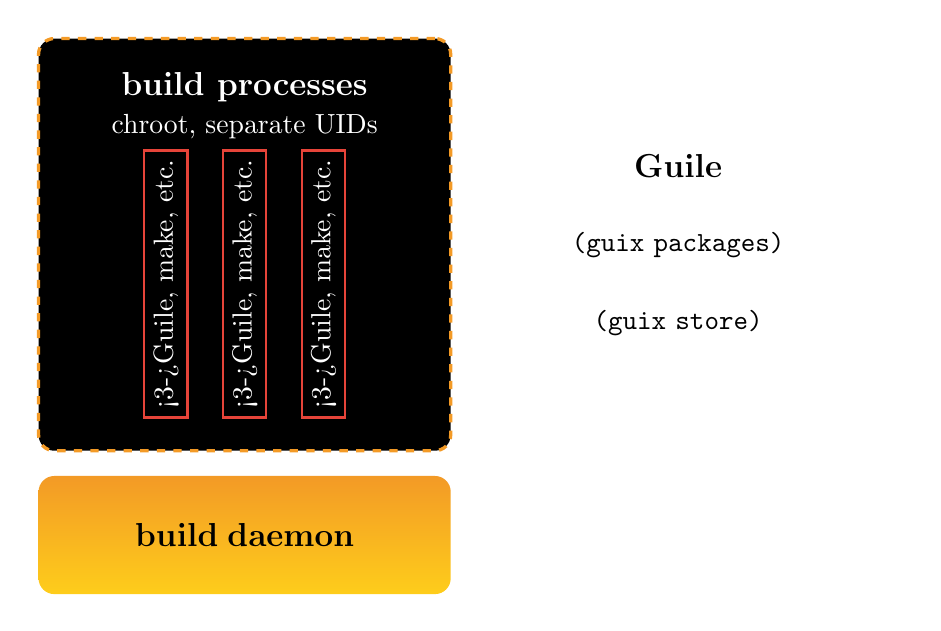
\begin{tikzpicture}[tools/.style = {
                        text width=35mm, minimum height=4cm,
                        text centered,
                        rounded corners=2mm,
                        fill=white, text=black
                      },
                      tool/.style = {
                        fill=white, text=black, text width=3cm,
                        text centered
                      },
                      daemon/.style = {
                        rectangle, text width=50mm, text centered,
                        rounded corners=2mm, minimum height=15mm,
                        top color=guixorange1,
                        bottom color=guixyellow,
                        text=black
                      },
                      builders/.style = {
                        draw=guixorange1, very thick, dashed,
                        fill=black, text=white, text width=5cm,
                        rounded corners=2mm,
                      },
                      builder/.style = {
                        draw=guixred2, thick, rectangle,
                        fill=black, text=white,
                        rotate=90
                      }]
    \matrix[row sep=3mm, column sep=1cm] {
      \node(builders)[builders, text height=5cm]{}
          node[fill=black, text=white] at (0, 2) {\large{\textbf{build processes}}}
          node[fill=black, text=white] at (0, 1.5) {chroot, separate UIDs}
          node[builder, onslide=<1-2>{black}] at (-1,-0.5) {\alert<3->{Guile}, make, etc.}
          node[builder, onslide=<1-2>{black}] at ( 0,-0.5) {\alert<3->{Guile}, make, etc.}
          node[builder, onslide=<1-2>{black}] at ( 1,-0.5) {\alert<3->{Guile}, make, etc.}; &
      \node[tools]{}
          node[fill=white, text=black] at (0, 1) {\large{\textbf{Guile}}}
          node[tool] at (0, 0) {\texttt{(guix packages)}}
          node(client)[tool] at (0, -1) {\texttt{(guix store)}};
      \\

      \node(daemon)[daemon]{\large{\textbf{build daemon}}}; &
      &
      \\
    };
  \end{tikzpicture}

  \begin{tikzpicture}[overlay]
    \path[very thick, draw=guixorange1]<2->
      (client.south) edge [out=-90, in=0, ->] node[below, sloped]{RPCs} (daemon.east);
    \path[->, very thick, draw=guixorange1]<3->
      (daemon) edge (builders);
  \end{tikzpicture}
\end{frame}


\begin{frame}[fragile]
  \begin{semiverbatim}
(\alert{use-modules} (guix packages) (guix store)
             (gnu packages base))

(define store
  (\alert<1>{open-connection}))

(package? hello)
=> \#t

\uncover<1->{(define drv (\alert{package-derivation} store hello))
\uncover<1->{drv
=> "/nix/store/xyz\textrm{...}-hello-2.8\alert{.drv}"

\uncover<1->{(build-derivations (list drv))
\textsf{\alert{... daemon builds/downloads package on our behalf...}}
\uncover<1->{=> "/nix/store/pqr\textrm{...}-hello-2.8"}}}}
  \end{semiverbatim}

  \begin{tikzpicture}[overlay]
    \node[rounded corners=4, text centered,
          fill=guixorange1, text width=3cm,
          inner sep=3mm, rotate=-5, opacity=.75, text opacity=1,
          drop shadow={opacity=0.5},
          at=(current page.center)] {
            \textbf{\large{Emacs + Geiser demo!}}
          };
  \end{tikzpicture}
\end{frame}


% \begin{frame}[fragile]{build expressions}
%   \begin{semiverbatim}
% (let* ((store   \tikz[baseline]{\node[anchor=base](conn){(open-connection)};})
%        (builder '(\tikz[baseline]{\node[anchor=base](builder){begin};}
%                    (mkdir \%output)
%                    (call-with-output-file
%                        (string-append \%output "/test")
%                      (lambda (p)
%                        (display '(hello guix) p)))))
%        (drv (\tikz[baseline]{\node[anchor=base](drv){\alert{build-expression->derivation}};}
%                store "foo" "x86\_64-linux"
%                builder
%                '(("HOME" . "/nowhere")))))
%   (\tikz[baseline]{\node[anchor=base](build){\alert{build-derivations}};} store (list drv)))
%   \end{semiverbatim}

%   % \begin{textblock}{6}(3, 2)
%   %   \tikz{\node<2>[fill=white, text=black](labelconn){connect to
%   %       the build daemon};}
%   % \end{textblock}

%   \begin{textblock}{6}(8, 2)
%     \tikz{\node<2>[fill=white, text=black](labelbuilder){build script,
%         to be eval'd in chroot};}
%   \end{textblock}

%   \begin{textblock}{4}(1, 6)
%     \tikz{\node<3>[fill=white, text=black, text width=4cm](labeldrv){compute derivation
%         for this builder, system, and env.~vars};}
%   \end{textblock}

%   \begin{textblock}{5}(1, 7)
%     \tikz{\node<4>[fill=white, text=black, text
%       width=4cm](labelguile){implicitly adds Guile as an input};}
%   \end{textblock}

%   \begin{textblock}{6}(1, 9)
%     \tikz{\node<5>[fill=white, text=black](labelbuild){build it!};}
%   \end{textblock}

%   \begin{tikzpicture}[overlay]
%     % \path[->, fill=white, thick]<2>(labelconn) edge (conn);
%     \path[->, fill=white, thick]<2>(labelbuilder) edge (builder);
%     \path[->, fill=white, thick]<3>(labeldrv) edge (drv);
%     \path[->, fill=white, thick]<4>(labelguile) edge (drv);
%     \path[->, fill=white, thick]<5>(labelbuild) edge (build);
%   \end{tikzpicture}
% \end{frame}

\begin{frame}[fragile]{}
  \begin{semiverbatim}
(package (\tikz[baseline]{\node(inherit)[anchor=base]{\alert{inherit}};} hello)
  (version "2.7")
  (source
    (origin
      (method url-fetch)
      (uri "mirror://gnu/hello/hello-2.7.tar.gz")
      (sha256
        (base32 "7dqw3...")))))
  \end{semiverbatim}

  \begin{textblock}{6}(7, 2)
    \tikz \node(labelinherit)[fill=white, text=black, text width=5.5cm]
      {copy fields from \texttt{hello} except for \texttt{version} and
        \texttt{source}};
  \end{textblock}
  
  \begin{tikzpicture}[overlay]
    \path[->] (labelinherit) edge (inherit);
  \end{tikzpicture}
\end{frame}

\begin{frame}[fragile]{}
  \begin{semiverbatim}
(define (static-package p)
  ;; Return a statically-linked variant of P.
  (package (\alert{inherit} p)
    (arguments
     `(\#:configure-flags '("--disable-shared"
                            "LDFLAGS=-static")
       ,@(package-arguments p)))))
  \end{semiverbatim}
\end{frame}

\begin{frame}[plain, fragile, t]
  \frametitle{workflow}

  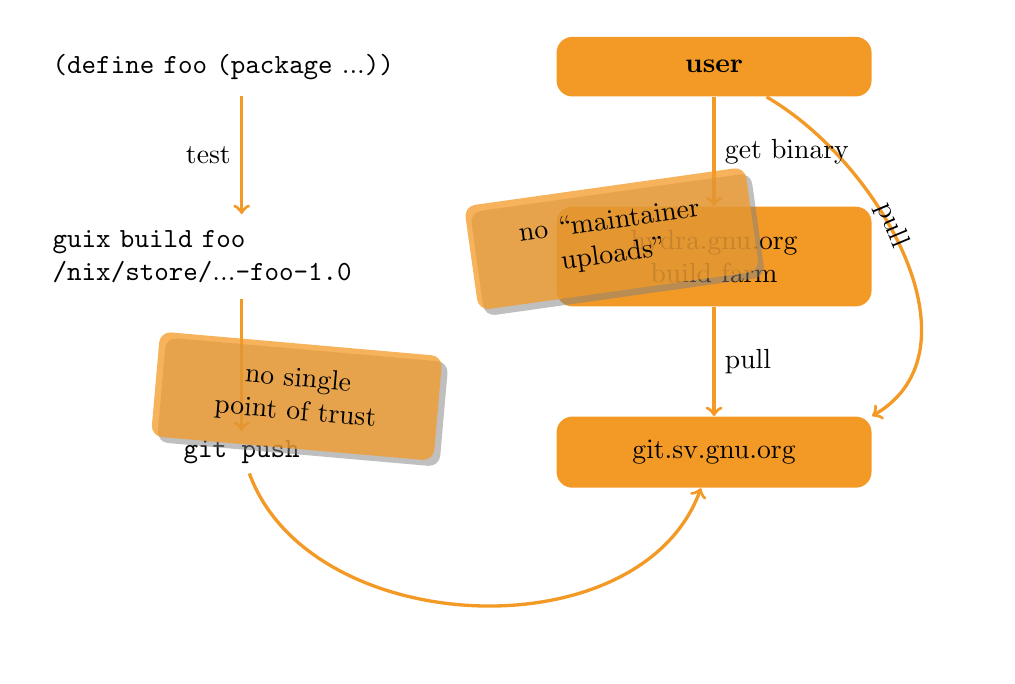
\begin{tikzpicture}[box/.style = {
                         rounded corners=2mm,
                         fill=white, text=black, text width=4.8cm,
                         inner sep=2mm
                      },
                      server/.style = {
                         text centered, rounded corners=2mm,
                         fill=guixorange1, text=black, text width=3.4cm,
                         inner sep=3mm
                      },
                      note/.style = {
                        rounded corners=4, text centered,
                        fill=guixorange1, text width=3cm,
                        inner sep=3mm, rotate=5, opacity=.75, text opacity=1,
                        drop shadow={opacity=0.5}
                      }]
    \matrix[row sep=1.4cm, column sep=1.4cm] {
      \node(def)[box]{\texttt{(define foo (package \textrm{...}))}};
      & \node(user)[server]{\textbf{user}};
      \\
      \node<2->(build)[box]{\texttt{guix build foo}
         \texttt{/nix/store/\textrm{...}-foo-1.0}};
      & \node<4-5>(hydra)[server]{hydra.gnu.org build~farm};
      \\
      \node<3->(push){\texttt{git push}};
      & \node<3->(savannah)[server]{git.sv.gnu.org}; \\
      \\
    };

    \path[->, very thick, draw=guixorange1]<2->
      (def) edge node[left]{test} (build);
    \path[->, very thick, draw=guixorange1]<3->
      (build) edge (push);
    \path[->, very thick, draw=guixorange1]<3->
      (push) edge[->, in=-110, out=-70] (savannah);
    \path[->, very thick, draw=guixorange1]<4-5>
      (hydra) edge node[right]{pull} (savannah);
    \path[->, very thick, draw=guixorange1]<4-6>
      (user) edge[in=30,out=-30] node[left, sloped]{pull}
      (savannah.north east);
    \path[->, very thick, draw=guixorange1]<5>
      (user) edge node[right]{get binary} (hydra);

    \node<7>[overlay, fill=black, opacity=.8, 
             text height=8cm, text width=11cm,
             at=(current page.center)] {};

    \node<7>[note, rotate=3] at (2,1) {no ``maintainer uploads''};
    \node<7>[note, rotate=-10] at (-2,-1) {no single point of trust};
  \end{tikzpicture}
\end{frame}

% \begin{frame}[fragile]{builder side of \texttt{gnu-build-system}}
%   \vspace{-0.4cm}
%   \begin{semiverbatim}
% (\alert{define} \%standard-phases
%   `((configure . ,configure)
%     (build . ,build)
%     ;; \textrm{...}
%     ))

% (\alert{define*} (gnu-build #:key (phases \%standard-phases)
%                     #:allow-other-keys
%                     #:rest args)
%   ;; Run all the PHASES in order, passing them ARGS.
%   (every (match-lambda
%           ((name . proc)
%            (format #t "starting phase `~a'~\%" name)
%            (let ((result (apply proc args)))
%              (format #t "phase `~a' done~\%" name)
%              result)))
%          phases))
%   \end{semiverbatim}
% \end{frame}

% \begin{frame}[fragile]{inserting a build phase}
%   \begin{semiverbatim}
% (define howdy
%   (\alert{package} (inherit hello)
%     (arguments
%       '(#:phases
%         (\tikz[baseline]{\node(alistcons)[anchor=base]{alist-cons-after};}
%           'configure 'change-hello
%           (lambda* (#:key system #:allow-other-keys)
%             (\tikz[baseline]{\node(subst)[anchor=base]{\alert<4>{substitute*}};} "src/hello.c"
%               (("Hello, world!")
%                (string-append "Howdy! Running on "
%                               system "."))))
%           \tikz[baseline]{\node(phases)[anchor=base]{\%standard-phases};})))))
%   \end{semiverbatim}

%   \begin{tikzpicture}[overlay]
%     \draw<2> (40pt, 145pt) [very thick, color=guixorange2, rounded corners=8pt]
%       arc (20:-40:-50pt and 110pt);
%     \node<2>[fill=white, text=black, text opacity=1, opacity=.7,
%           rounded corners=2mm, inner sep=5mm]
%       at (7, 4) {\textbf{builder-side expression}};
%   \end{tikzpicture}

%   \begin{textblock}{5}(1, 9)
%     \tikz{\node<3>[fill=white, text=black](labelphases){configure, build, check, install};}
%   \end{textblock}

%   \begin{textblock}{5}(8, 5)
%     \tikz{\node<3>(labelalistcons)[fill=white, text=black]{add a phase
%         before \texttt{configure}};}
%   \end{textblock}

%   \begin{textblock}{5}(5, 5)
%     \tikz{\node<4>(labelsubst)[fill=white, text=black]{patch things up à
%         la \texttt{sed}};}
%   \end{textblock}

%   \begin{tikzpicture}[overlay]
%     \path[->, fill=white, thick]<3>(labelphases) edge (phases);
%     \path[->, fill=white, thick]<3>(labelalistcons) edge (alistcons);
%     \path[->, fill=white, thick]<4>(labelsubst) edge (subst);
%   \end{tikzpicture}
% \end{frame}

\begin{frame}[plain]
  \begin{centering}
    \Huge{\textbf{\alert{boot time!}}}
  \end{centering}
\end{frame}

\begin{frame}[plain, fragile]
  \begin{semiverbatim}
(define my-config
  (\alert{operating-system}
   (host-name "gnubox")
   (timezone "Europe/Paris")
   (locale "en\_US.UTF-8")\only<2->{
   (\alert{initrd} \only<2>{(qemu-initrd)}\only<3>{(expression->initrd \textrm{...})})}
   (users (list (user-account
                 (name "ludo")
                 (uid 1000) (gid 100)
                 (comment "Hello, this is me!")
                 (home-directory "/home/ludo"))))
   (packages (list coreutils bash grep sed
                   findutils inetuils
                   guile-2.0
                   dmd guix
                   procps psmisc
                   zile less))))
  \end{semiverbatim}
\end{frame}

\begin{frame}[plain, fragile]
  \begin{semiverbatim}
\small{
(\alert{expression->initrd}
 '(begin
    (mkdir "/proc")
    (mount "none" "/proc" "proc")

    ;; Load Linux kernel modules.
    (let ((slurp (lambda (module)
                   (call-with-input-file
                       (string-append "/modules/" module)
                     get-bytevector-all))))
      (for-each (compose load-linux-module slurp)
                (list "md4.ko" "ecb.ko" "cifs.ko")))

    ;; Turn eth0 up.
    (let ((sock (socket AF_INET SOCK_STREAM 0)))
      (set-network-interface-flags sock "eth0" IFF_UP))

    ;; At last, the warm and friendly REPL.
    (start-repl)))
}
  \end{semiverbatim}

  \begin{tikzpicture}[overlay]
    \node[rounded corners=4, text centered,
          fill=guixorange1, text width=3cm,
          inner sep=3mm, rotate=-10, opacity=.75, text opacity=1,
          drop shadow={opacity=0.5}] at (9,8) {
            \textbf{\large{boot to Guile!}}
          };
  \end{tikzpicture}
\end{frame}

\begin{frame}[plain, fragile]
  \begin{semiverbatim}
(define my-config
  (\alert{operating-system}
   (host-name "gnubox")
   (timezone "Europe/Paris")
   (locale "en\_US.UTF-8")\only<2>{
   (\alert{services}
     (list (mingetty-service "tty1"
             #:motd (text-file "motd" "This is tty One."))
           (mingetty-service "tty2")
           (syslog-service)
           (nscd-service)))}
   (users (list (user-account
                 (name "ludo")
                 (uid 1000) (gid 100)
                 (comment "Hello, this is me!")
                 (home-directory "/home/ludo"))))
   (packages (list coreutils bash grep sed
                   \textrm{...}))))
  \end{semiverbatim}
\end{frame}

\begin{frame}[plain, fragile]
  \begin{semiverbatim}
# deco status dmd
Started: (term-tty1 term-tty2 nscd syslog)
Stopped: ()

# deco stop nscd
Service nscd has been stopped
  \end{semiverbatim}

  \begin{tikzpicture}[overlay]
    \node[rounded corners=4, text centered,
          fill=guixorange1, text width=3cm,
          inner sep=3mm, rotate=-10, opacity=.75, text opacity=1,
          drop shadow={opacity=0.5}] at (8,5) {
            \textbf{\large{PID 1 is GNU dmd!}}
          };
  \end{tikzpicture}
\end{frame}

\begin{frame}
  \frametitle{GNU dmd in a nutshell}

  \large{
  \begin{itemize}
    \item born in \alert{2003}, revived in 2013 :-)
    \item dependency-based service manager
    \item<2-> \texttt{dmd} is PID 1, \texttt{deco} is a client
    \item<3-> written in \alert{Guile} Scheme
    \item<3-> dynamic, extensible, etc.
  \end{itemize}}
\end{frame}

%%%%%%%%%%%%%%%%%%%%%%%%%%%%%%%%%%%%%%%%%%%%%%%%%%%%%%%%%%%%%%%%%%%%%%%%%%%%%%%%
\begin{frame}[plain]
  \begin{centering}
    \Huge{\textbf{Liberating.}}
  \end{centering}
\end{frame}

\begin{frame}[plain]
  \begin{tikzpicture}[overlay]
    % http://www.gnu.org/graphics/runfreegnu.html
    \node [at=(current page.center), inner sep=0mm]
    {\includegraphics[width=\paperwidth]{images/runfreerungnu-white}};
  \end{tikzpicture}
\end{frame}

\begin{frame}[fragile]{}

  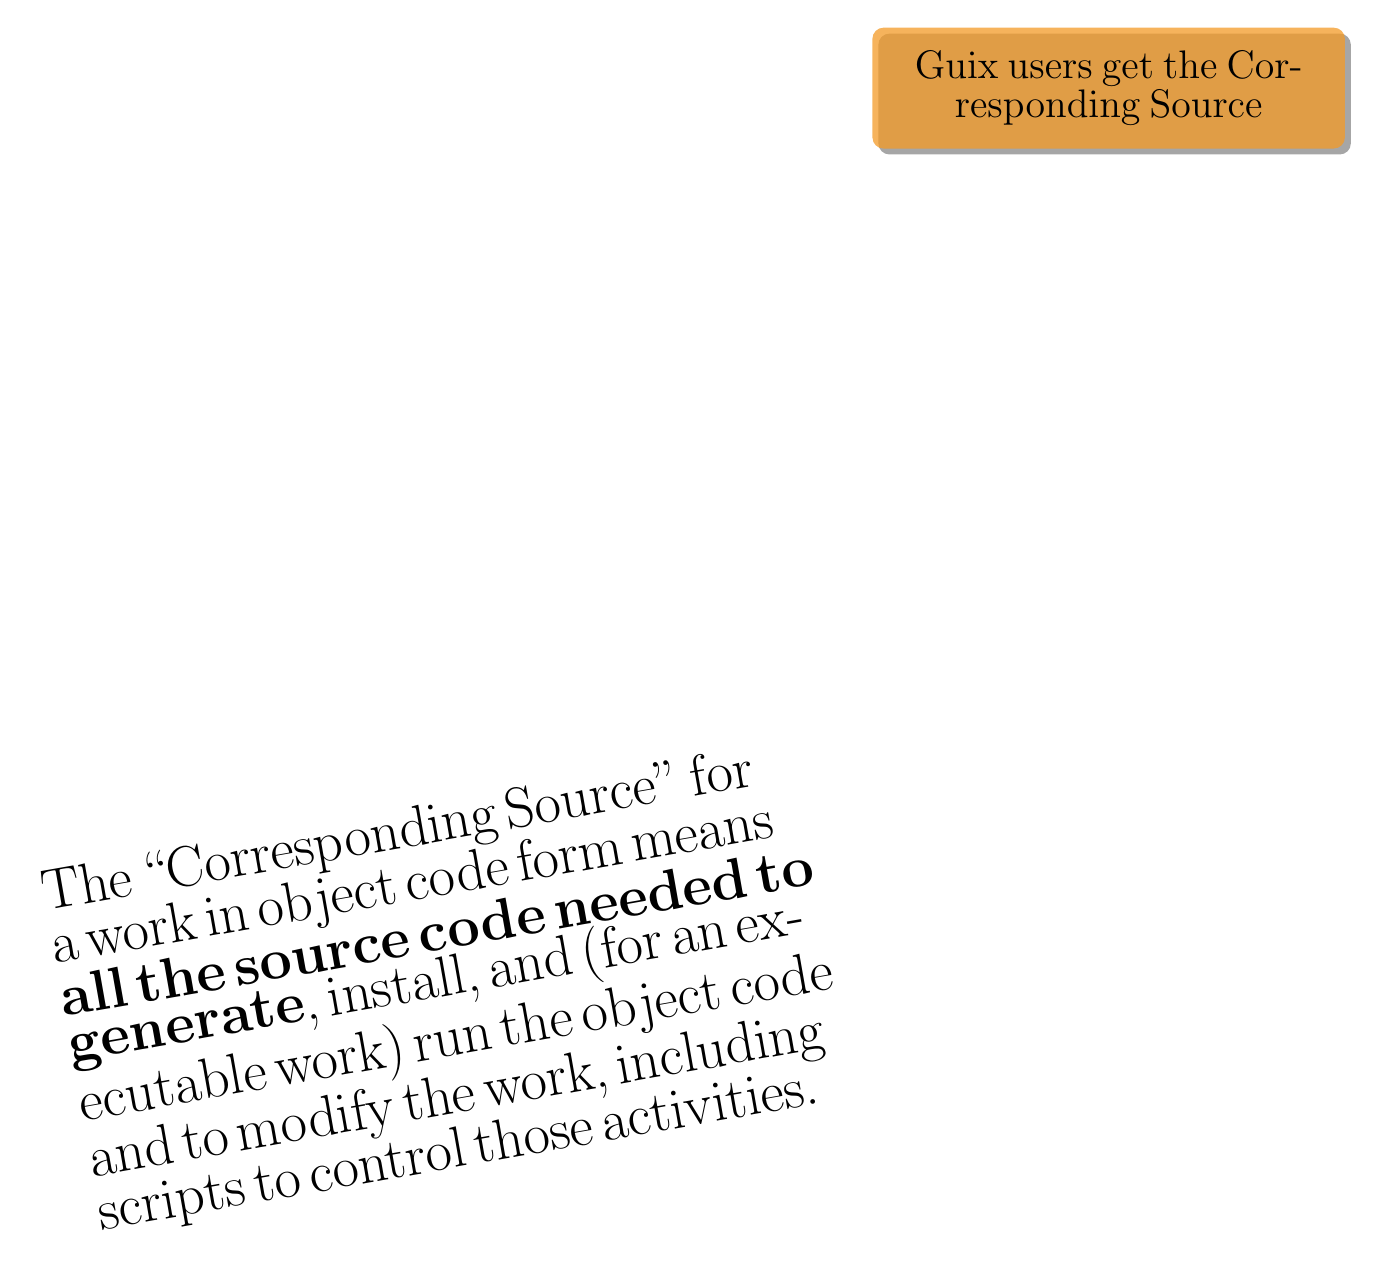
\begin{tikzpicture}
    \node[rotate=10, text width=10cm]{ \huge{\textrm{The
          ``Corresponding Source'' for a work in object code form means
          \alert{\textbf{all the source code needed to generate}},
          install, and (for an executable work) run the object code and
          to modify the work, including scripts to control those
          activities.}}};
    \node<2->[rounded corners=4, text centered,
          fill=guixorange1, text width=5.4cm,
          inner sep=3mm, opacity=.75, text opacity=1,
          drop shadow={opacity=0.7},
          at=(current page.center)]{%
            \Large{Guix users get the
              Corresponding Source}};
  \end{tikzpicture}
\end{frame}

\begin{frame}[plain]

  \begin{tikzpicture}[overlay]
    \node (hellobuilddeps) [at=(current page.center), inner sep=0] {%
      \includegraphics[width=\paperwidth]{images/hello-buildtime-deps}%
    };

    \node<2-> (bootbinlabel) at (6cm,2.5cm) {%
      \textbf{bootstrap} binaries%
    };
    \node<1> (hellobuilddepslabel) at (6cm,-4.5cm) {%
      build-time dependencies of GNU Hello%
    };
    \path[->]<1> (hellobuilddepslabel.north) edge [bend left, in=180] (hellobuilddeps.south);
    \path[->]<2> (bootbinlabel.south) edge [bend left, in=180] (hellobuilddeps.north);
    \path[->]<3> (hellobuilddepslabel.north)
       edge [bend right, in=-90, out=-90, very thick]
       node [below, sloped] {\large{can we close the loop?}}
       (hellobuilddeps.north);
  \end{tikzpicture}
\end{frame}

% \begin{frame}[plain]
%   \begin{tikzpicture}[overlay]
%     % http://innovation-al.com/wp-content/uploads/2013/03/Boots.jpg
%     % http://en.wikipedia.org/wiki/File:Dr_Martens,_black,_old.jpg
%     \node [at=(current page.center), inner sep=0mm]
%     {\includegraphics[width=1.1\paperwidth]{images/boots-with-strap}};

%     \node at (3cm, 3cm) [text=black](label) {%
%       \Large{\textbf{boot strap}}%
%     };
%     \path[very thick, draw=black] (label.east)
%       edge [bend right, out=10, in=170, ->] (5.4cm, 2.7cm);
%   \end{tikzpicture}
% \end{frame}

% \begin{frame}[fragile]
%   \begin{semiverbatim}
% (\alert{origin}
%   (method \tikz[baseline]{\node(fetch)[anchor=base]{url-fetch};})
%   (uri (string-append "mirror://gnu/gcc/gcc-"
%                       version "/gcc-" version
%                       ".tar.bz2"))
%   (sha256 (base32 "1hx9\textrm{...}")))
%   \end{semiverbatim}

%   \begin{tikzpicture}[overlay]
%     \node<2->(labelfetch)[fill=white, text=black] at (4, 5)
%       {use Guile HTTP(S)/FTP client};
%     \path[->, fill=white, thick]<2-> (labelfetch) edge (fetch);

%     \node<3->[overlay, rounded corners=4, text centered,
%             minimum size=10mm, fill=guixorange1, text width=5cm,
%             inner sep=3mm, rotate=2, opacity=.75, text opacity=1,
%             drop shadow={opacity=0.5}] at (5, 1) {
%               \textbf{how is the very first tarball downloaded?}
%             };
%   \end{tikzpicture}
% \end{frame}

% \begin{frame}[fragile]{bootstrapping the distribution}
%   \begin{enumerate}
%     \setcounter{enumi}{-1}
%     \item<1-> statically-linked binaries of \texttt{mkdir}, \texttt{tar},
%       \texttt{xz}, \texttt{bash}, and Guile
%     \item<2-> derivation runs Bash script to untar Guile
%     \item<3-> use Guile to download statically-linked binaries of GCC,
%       Binutils, libc, Coreutils et al., and Bash
%     \item<4-> use that to build GNU~Make
%     \item<5-> build a tool chain independent of the bootstrap binaries
%   \end{enumerate}

%   \begin{tikzpicture}[overlay]
%     % \draw<6-> (100pt, 115pt) [very thick, color=guixorange2, rounded corners=8pt]
%     %   arc (90:270:10pt);
%     \node<6->[overlay, rounded corners=4, text centered,
%             minimum size=10mm, fill=guixorange1, text width=8cm,
%             inner sep=3mm, rotate=2, opacity=.75, text opacity=1,
%             drop shadow={opacity=0.5}] at (5, 1) {
%               \textbf{what led to the binaries in step 0?}
%             };
%   \end{tikzpicture}
% \end{frame}

\begin{frame}[fragile]
  \begin{semiverbatim}
\$ guix build bootstrap-tarballs
/nix/store/\textrm{...}-bootstrap-tarballs-0
  \end{semiverbatim}
  \uncover<2->{porting to new arches:}
  \begin{semiverbatim}
    \uncover<2->{
\$ guix build bootstrap-tarballs \\
     \alert{--target}=mips64el-linux-gnuabi64
    }
  \end{semiverbatim}
\end{frame}

\begin{frame}[plain]
  \LARGE{Does this binary \alert{\textbf{correspond}}\\[3mm]
    to that source?}
\end{frame}

\begin{frame}[fragile]
  \frametitle{}

  \begin{semiverbatim}
\$ guix build guile
\uncover<2->{/nix/store/\tikz[baseline]{\node[anchor=base](nixhash){\alert<2>{h2g4sc09h4...}};}-guile-2.0.9}

\uncover<3->{\$ \alert<3>{guix gc --references /nix/store/...-guile-2.0.9}
/nix/store/4jl83jgzaac...-glibc-2.17
/nix/store/iplay43cg58...-libunistring-0.9.3
/nix/store/47p47v92cj9...-libffi-3.0.9
/nix/store/drkwck2j965...-gmp-5.0.5
...}
  \end{semiverbatim}

  \begin{tikzpicture}[overlay]
    \node<2>(labelnixhash) [fill=white, text=black] at (4cm, 2cm) {%
      hash of \textbf{all} the dependencies};
    \path[->]<2>(labelnixhash.north) edge [bend left, in=180, out=-45] (nixhash.south);

    \draw<4> (-10pt, 105pt) [very thick, color=guixorange2, rounded corners=8pt]
      arc (10:-50:-50pt and 110pt);
    \node<4>[fill=white, text=black, text opacity=1, opacity=.7,
          rounded corners=2mm, inner sep=5mm]
      at (7, 2) {\textbf{(nearly) bit-identical for everyone}};
  \end{tikzpicture}

\end{frame}


\begin{frame}
  \frametitle{controlled build environment}

  \begin{enumerate}
    \item one directory \alert{\textbf{per installed package}}
    \item \alert{\textbf{immutable}} installation directories
    \item undeclared dependencies \alert{\textbf{invisible}} to the build process
    \item \alert{\textbf{isolated build}}: chroot, container, etc.
  \end{enumerate}

\end{frame}


% \begin{frame}
%   \frametitle{functional packaging summarized}

%   \vspace{1cm}
%   \begin{itemize}
%     \item \alert{\bf immutable} software installations
%     \item builds/installs have \alert{\bf no side effects}
%     \item build \& deployment $\equiv$ \alert {\bf calling a build function}
%     \item the store $\equiv$ \alert{\bf memoization}
%     \item garbage collection...
%   \end{itemize}
% \end{frame}


\begin{frame}[plain]
  \begin{tikzpicture}[overlay]
    % http://ergoemacs.org/emacs/i/Richard_Stallman_and_Julian_Assange_2013-07-12.jpg
    \node [at=(current page.center), inner sep=0mm]
    {\includegraphics[height=\paperheight]{images/Stallman-Assange-2013-07-12}};
  \end{tikzpicture}
\end{frame}

\begin{frame}[plain]
  \LARGE{do not \alert{trust} a single\\ binary provider}

  \uncover<2>{
  \vspace{1cm}
  % \hfill{\url{https://blog.torproject.org/blog/deterministic-builds-part-one-cyberwar-and-global-compromise}}
  \textrm{\LARGE{Deterministic Builds: Integrity\\
      through Decentralization}}

  \vspace{0.6cm}
  \hfill{\large{-- Mike Perry}}}
\end{frame}


%%%%%%%%%%%%%%%%%%%%%%%%%%%%%%%%%%%%%%%%%%%%%%%%%%%%%%%%%%%%%%%%%%%%%%%%%%%%%%%%


% \begin{frame}[fragile]{building packages}
%   \begin{semiverbatim}
% \$ \alert<1>{guix build}\only<3->{ --\alert{target}=armel-linux-gnueabi} hello
% \uncover<2->{The following derivations will be built:
%    /nix/store/\only<1-2>{4gy79}\only<3>{1gm99}\textrm{...}-\only<1-2>{gawk-4.0.0}\only<3>{gcc-armel-linux-gnu-4.8.1}.drv
%    /nix/store/\only<1-2>{7m2r9}\only<3>{71ah1}\textrm{...}-hello-2.8.drv
% \textrm{...}
% \alert{/nix/store/\only<1-2>{71aj1}\only<3->{7m2r9}\textrm{...}-hello-2.8}
% }
% \end{semiverbatim}
% \end{frame}

% \begin{frame}[fragile]{customized package declaration}
%   \begin{semiverbatim}
%     \vspace{-1.3cm}
%     \small{
% (define guile-1.8
%   (\alert{package} \textrm{...}
%    (\alert{arguments}
%      '(\alert<1>{#:configure-flags} '("--disable-error-on-warning")
%        \uncover<2->{\alert<2>{#:patches} (list (assoc-ref %build-inputs "patch/snarf"))}

%        \uncover<3->{
%        \alert<3-4>{#:phases}
%          (\tikz[baseline]{\node[anchor=base](alistcons){alist-cons-before 'configure 'patch-search-path};}
%             (lambda* (#:key outputs #:allow-other-keys)
%               (\tikz[baseline]{\node[anchor=base](subst){\alert<5>{substitute*}};} "libguile/dynl.c"
%                 (("lt_dlinit.*\$" match)
%                  (format \#f
%                    "  ~a~\%  lt\_dladdsearchdir(\\"~a/lib\\");~\%"
%                    match (assoc-ref outputs "out")))))
%             \tikz[baseline]{\node[anchor=base](phases){\alert<3-4>{\%standard-phases}};})}))
%    (inputs `(\uncover<2->{("\alert<2>{patch/snarf}" "guile-1.8.patch")}
%              ("gawk" ,gawk)
%              ("readline" ,readline)))

%    ...
%    }
%   \end{semiverbatim}

%   \begin{textblock}{5}(1, 9)
%     \tikz{\node<3-4>[fill=white, text=black](labelphases){configure, build, check, install};}
%   \end{textblock}

%   \begin{textblock}{5}(8, 5)
%     \tikz{\node<4>(labelalistcons)[fill=white, text=black]{add a phase
%         before \texttt{configure}};}
%   \end{textblock}

%   \begin{textblock}{5}(5, 5)
%     \tikz{\node<5>(labelsubst)[fill=white, text=black]{patch things up à
%         la \texttt{sed}};}
%   \end{textblock}

%   \begin{tikzpicture}[overlay]
%     \path[->, fill=white, thick]<3-4>(labelphases) edge (phases);
%     \path[->, fill=white, thick]<4>(labelalistcons) edge (alistcons);
%     \path[->, fill=white, thick]<5>(labelsubst) edge (subst);
%   \end{tikzpicture}
% \end{frame}


%%%%%%%%%%%%%%%%%%%%%%%%%%%%%%%%%%%%%%%%%%%%%%%%%%%%%%%%%%%%%%%%%%%%%%%%%%%%%%%%
\begin{frame}[plain]
  \begin{centering}
    \Huge{\textbf{Lively!}}
  \end{centering}
\end{frame}

\begin{frame}[plain]
  \vspace{2cm}
  \textrm{\LARGE{%
      Shipping is a feature.\\
      A really important feature.
    }}
  
  \vspace{2cm}
  \hfill{-- Joel Spolsky}
\end{frame}

\begin{frame}{timeline}
  \begin{itemize}
    \item July 2012 --- GHM, Düsseldorf
    \item Nov. 2012 --- dubbed GNU
    \item{Jan. 2013 --- \alert{0.1}}
    \item{Feb. 2013 --- Boot-to-Guile}
    \item{May 2013 --- \alert{0.2}}
    \item{June 2013 --- European Lisp Symposium}
    \item{July 2013 --- \alert{0.3}, cross-compilation, debug info, etc.}
    \item{27 Sep. 2013 --- \alert{0.4}, with VM image}
    \item{Dec. 2013 --- \alert{GNU dmd} 0.1}
    \item{Dec. 2013 --- \alert{0.5}, system config, mips64, 600 packages}
  \end{itemize}
\end{frame}

\begin{frame}{status}
  \large{
  \begin{itemize}
    \item full-featured package manager
    \item self-contained distro, 600+ packages, 3 platforms
    \item binaries built \& served at \url{http://hydra.gnu.org}
    \item tooling: auto-update, sync descriptions with GNU, etc.
    \item l10n: 4 languages!
  \end{itemize}}
\end{frame}

\begin{frame}[plain]
  \begin{tikzpicture}[overlay]
    % http://www.ohloh.net/p/gnuguix
    \node [at=(current page.center), inner sep=0mm]
    {\includegraphics[width=0.9\paperwidth]{images/ohloh-commits}};
  \end{tikzpicture}
\end{frame}

% \begin{frame}{status}
%   \begin{itemize}
%     \item{community!
%         \begin{itemize}
%           \item<2-> 4+ regular contributors
%         \end{itemize}}
%     \item<3-> active repo, active mailing list, IRC channel
%     \item<3-> \url{http://bugs.gnu.org/guix} + \texttt{guix-devel@gnu.org}
%   \end{itemize}
% \end{frame}

\begin{frame}[plain]

  \begin{tikzpicture}[remember picture, overlay]
    \node [at=(current page.center), inner sep=0pt]
      {\includegraphics[width=\paperwidth]{images/ohloh-summary}};
    % \fill (0,0) circle (2pt);
    % \fill (10,0) [fill=red] circle (2pt);
    % \fill (0,4) [fill=green] circle (2pt);
    % \fill (10,4) [fill=blue] circle (2pt);
    \path[very thick, draw=red] (3.6cm, -3.5cm)
      edge [bend left, in=-60, out=-60] (6.6cm,-2.9cm);
  \end{tikzpicture}
\end{frame}

\begin{frame}{thanks for the code, bug reports, and ideas!}

  \begin{itemize}
    \item Eric Bavier, John Darrington, Eelco Dolstra~\& the Nix crew,
      Andreas Enge, Guy Grant, Nikita Karetnikov, Aljosha Papsch, Cyril
      Roelandt, Alex Sassmannshausen, Sree Harsha Totakura, David
      Thompson, Mark H. Weaver
    \item Lluís Batlle i Rossell, Felipe Castro, Daniel Clark,
      Alexandru Cojocaru, Aleix Conchillo Flaqué, Rafael Ferreira,
      Christian Grothoff, Jeffrin Jose, Kete, Matthew Lien, Niels
      Möller, Yutaka Niibe, Cyrill Schenkel, Jason Self, Alen Skondro,
      Matthias Wachs, Zerwas
  \end{itemize}
\end{frame}

\begin{frame}{the road to 1.0}
  \Large{
    \begin{enumerate}
    \item<1-> simple \textbf{installer} ISO image (real soon)
    \item<2-> \textbf{infrastructure}: get a real build farm
    \item<3-> packages, packages, \textbf{packages}!
    \end{enumerate}
  }

\end{frame}

\begin{frame}[plain]

  \vspace{0.7cm}
  \Large{
    \begin{itemize}
    \item \textbf{install Guix} atop your current distro
    \item \textbf{use it}, report bugs, add packages
    \item help with the \textbf{infrastructure} + admin
    \item share your \textbf{ideas}!
    \end{itemize}
  }

  \begin{textblock}{5}(7,8)
    \tikz
    \node[overlay, rounded corners=4, text centered,
          minimum size=10mm, fill=guixorange1, text width=5cm,
          inner sep=3mm, rotate=-7, opacity=.75, text opacity=1,
          drop shadow={opacity=0.5}] at (3, 3) {
            \textbf{your help needed!}
          };
  \end{textblock}
\end{frame}

\begin{frame}{}

\vfill{
  \vspace{6.5cm}
  \hfill{\includegraphics[width=0.3\textwidth]{images/guix-logo-white}}\\[0.2cm]
  \texttt{ludo@gnu.org} \hfill{\alert{\url{http://gnu.org/software/guix/}}}
}

\end{frame}

\begin{frame}{credits}
  \small{
  \begin{itemize}
  \item GNU Guix logo, GFDL, \url{http://gnu.org/s/guix/graphics}
  \item ``GNU marketing dept.'' picture by the Free Software Foundation,
    \url{http://www.fsf.org/news/gnu-comes-bearing-gifts-draws-shoppers-from-windows-store}
  \item ``Lisp is over half a century old'', \url{http://xkcd.com/297/}
  \item ``Run free, run GNU'', GFDL,
    \url{http://www.gnu.org/graphics/runfreegnu.html}
  \item Stallman \& Assange,
    \url{http://ergoemacs.org/emacs/i/Richard_Stallman_and_Julian_Assange_2013-07-12.jpg}
  \item commit stats \& project summary,
    \url{http://www.ohloh.net/p/gnuguix}
  \end{itemize}
  }
\end{frame}

\begin{frame}{}

  \begin{textblock}{12}(2, 8)
    \tiny{
      Copyright \copyright{} 2010, 2012, 2013, 2014 Ludovic Courtès \texttt{ludo@gnu.org}.

      Picture of user environments is: \\
      Copyright \copyright{} 2009 Eelco Dolstra \texttt{e.dolstra@tudelft.nl}.

      Copyright of other images included in this document is held by
      their respective owners.
      \\[3.0mm]
      This work is licensed under the \alert{Creative Commons
        Attribution-Share Alike 3.0} License.  To view a copy of this
      license, visit
      \url{http://creativecommons.org/licenses/by-sa/3.0/} or send a
      letter to Creative Commons, 171 Second Street, Suite 300, San
      Francisco, California, 94105, USA.
      \\[2.0mm]
      At your option, you may instead copy, distribute and/or modify
      this document under the terms of the \alert{GNU Free Documentation
        License, Version 1.3 or any later version} published by the Free
      Software Foundation; with no Invariant Sections, no Front-Cover
      Texts, and no Back-Cover Texts.  A copy of the license is
      available at \url{http://www.gnu.org/licenses/gfdl.html}.
      \\[2.0mm]
      % Give a link to the 'Transparent Copy', as per Section 3 of the GFDL.
      The source of this document is available from
      \url{http://git.sv.gnu.org/cgit/guix/maintenance.git}.
    }
  \end{textblock}
\end{frame}


\end{document}

% Local Variables:
% coding: utf-8
% comment-start: "%"
% comment-end: ""
% ispell-local-dictionary: "american"
% compile-command: "rubber --pdf guix-fosdem-2014.tex"
% End:
